\section{Recursion}
\label{sec:recursion}

Recursion is the process of repeating items in a self-similar way. It
is a concept that appears often in computer science and other branches
of mathematics (e.g.~number theory, fractals), but it has also
attracted some interest from fields like the arts in recent times
(look up ``recursive images'' on your favourite search engine!). 

In programming, the most basic form of recursion happens when a method
calls itself. This is something that can be done in any modern 
programming language, including
Java, Java Decaf, and Groovy. 

% THIS EXAMPLE IS NOT GOOD ANYMORE NOW THAT RECURSION-1 COMES BEFORE
% DATA STRUCTURES (so that they understand recursive traversal of
% lists and trees). 
% 
% We have already seen some examples of recursive
% calls, e.g.~when we tried to calculate the depth of a tree in one of
% the exercises: 
%
% \begin{verbatim}
% 01    // Method of class Node/Tree
% 02    public int depth() {
% 03        int leftDepth = 0;
% 04        if (left != null) {
% 05            leftDepth = left.depth();
% 06        }
% 07        int rightDepth = 0;
% 08        if (right != null) {
% 09            rightDepth = right.depth();
% 10        }
% 11        int depthBelow = Math.max(leftDepth, rightDepth);
% 12        return 1 + depthBelow;
% 13    }
% \end{verbatim}
%
% This method calls itself twice (lines 05 and 09) before it can return
% a value to the caller (line~12). 
% In order to return the depth under a node in a binary tree,
% the depth under the left branch is calculated (if it exists, otherwise
% it is zero), then the depth under the right 
% branch (if it exists), and then the
% result is the maximum of both depths plus one. The method
% \verb+depth()+ is \emph{recursive}. 
%
% In this section we are going to
% learn more about how recursion works, when it is a good idea to use
% it, and what are the possible pitfalls and how to avoid them. 

\label{neverends}
\begin{verbatim}
01    public int countForeverUp(int previousCount) {
02        int newCount = previousCount + 1;
03        printLine(newCount);
04        countForeverUp(newCount); // the method calls itself
05    }
\end{verbatim}

We are going to learn now the basic of recursive programming. This
will help us understand a bit deeper how the stack works when a method
is called, and it will also be useful when we start learning about
dynamic data structures. We will go into the more advanced aspects of
recursion during the second half of the course. 

\subsection{Classical examples: factorials and Fibonacci numbers}
\label{sec:class-exampl-fact}

\subsubsection{Factorials}

The factorial of a natural number is represented with an exclamation
mark (!) and defined\footnote{If you maths-inclined and would like to see
  how the factorial of a \emph{real} (non-natural) number is defined, search for the
  $\Gamma$ (gamma) function.} as:  

$$ n! = n \times (n - 1) \times (n - 2) \times \ldots \times 2 \times 1 $$

This definition makes it very easy to write a function that calculates
the factorial of a number recursively: 

\begin{verbatim}
01    public int factorial(int n) {
02        if (n == 1) {
03          return 1; 
04        } else {
05            int result = n * factorial(n-1);
06            return result;
07        }
08    }
\end{verbatim}

%%% No "static" at this point. On year-2 static is introduced after
%%% recursion. 
% Note that the method is static because it has no side effects,
% i.e.~it is a \emph{pure function}. 
If the argument is 1, the function returns 1 (because 
\mbox{1! = 1).} 
Otherwise, the function returns the argument multiplied by the
factorial of the argument minus one; that function call will in turn
return its argument (n-1) multiplied by the factorial of its argument
minus one (n-2); and so on. If we want to calculate the factorial
of~4, the resulting calculations look like this: 

\begin{equation*}
 \begin{aligned}
  \textrm{factorial(4)} & ~~~~~~~~~~~ \verb++\\
  \textrm{4 } \times \textrm{ factorial(3)} & ~~~~~~~~~~~ \textrm{(line 05)} \\
  \textrm{4 } \times \textrm{ (3 } \times \textrm{ factorial(2))} &  ~~~~~~~~~~~ \textrm{(line 05)} \\
  \textrm{4 } \times \textrm{ (3 } \times \textrm{ (2 } \times  \textrm{ factorial(1)))} & ~~~~~~~~~~~ \textrm{(line 05)}\\
  \textrm{4 } \times \textrm{ (3 } \times \textrm{ (2 } \times  \textrm{ 1))} & ~~~~~~~~~~~ \textrm{(line 03)}\\
  \textrm{4 } \times \textrm{ (3 } \times \textrm{ 2)} & ~~~~~~~~~~~ \textrm{(line 06)} \\
  \textrm{4 } \times \textrm{ 6} & ~~~~~~~~~~~ \textrm{(line 06)}\\
  \textrm{24} & ~~~~~~~~~~~ \textrm{(line 06)}\\
 \end{aligned}
\end{equation*}

\subsubsection{Fibonacci numbers}

Another classical example of recursivity are the sequence of Fibonacci
numbers\footnote{Fibonacci numbers were discovered by Italian mathematician
Leonardo di Pisa (known as Fibonacci) in the early 13$^{th}$ century
as an ideal solution to the growth of the population of rabbits. The
sequence of Fibonacci numbers starts as 1, 1, 2, 3, 5, 8, 13, 21, 34,
55, 89\ldots Fibonacci introduced arabic numerals to the West, so
thanks to him we can write 2989 instead of MMCMLXXXVIII.}, where every
number is the addition of the preceding two. 
In other words, Fibonacci numbers are defined recursively as:

$$ F(n) = 
  \begin{cases} 
    1,               & \mbox{if } n < 2 \\ 
    F(n-1) + F(n-2), & \mbox{if } n \ge 3
  \end{cases}
$$

They have many applications in computer science and biology, among
other fields. As they are defined recursively, a recursive method to
calculate the n$^{th}$ Fibonacci number is quite straightforward to
write: 

\begin{verbatim}
    public int fib(int n) {
        if ((n == 1) || (n == 2)) {
          return 1; 
        } else {
            int result = fib(n-1) + fib(n-2); // method calls itself
            return result;
        }
    }
\end{verbatim}

\subsection{How does recursion work?}
\label{sec:how-does-recursion}

% How does it work in simple terms?
% Define a base case, trivial (i.e. 0-bricks wall)
% Define how one case depends on a former case (a wall with all but
% one brick)
% ...I am not sure this works well in writing...

Recursion works as any other method call. There is no magic. When a
statement in Java calls a method, the same process is always 
followed: 

\begin{enumerate}
\item A new level is added to the stack.
\item The values given by the caller code are copied into the
  parameters in the new level.
\item The \emph{hidden parameter} ``this'' is also copied into the stack,
  pointing to the object where the method is called. It is accessed
  with the reserved keyword \verb+this+ (e.g.~\verb+this.name = name+).
\item The code of the method is executed as usual. Any new local
  variable is created on the new level in the stack. 
\item When a \verb+return+ statement is reached, the corresponding
  return value (if any) is stored.
\item The level in the stack is wiped out, and its local variables
  (and parameter values) forgotten. The return value (if any) is
  returned to the original caller code (and usually assigned to a
  variable).
\end{enumerate}

This does not change in the case of a recursive call. If we take the
calculation of 4! (factorial of 4) that we used before as an example, 
the computer stack changes are
represented if Figure~\ref{fig:fact}. First, a level is added to the
stack and the parameters are copied (only \verb+n+ in this 
case\footnote{The \emph{hidden parameter ``this'' is not 
shown for clarity}}, with
value~4). The code of the method is executed line by line: as \verb+n+
is not equal to~1 (line~2), 
a new local variable \verb+result+ is created (line~5); its value
is~1 plus the result of calling a method (line~5). 
A new level is added to the
stack, and the parameter values are copied (only \verb+n+ again, but
this time with value~3). A local variable \verb+result+ is created and
then the method is called again (line~5) 
so we need to add a new level in the
stack. The process is repeated once more, and we call the method with
a value of 1 for \verb+n+. At this point, 
the method returns~1 (line~3). Then
the calling method can finally calculate the value of \verb+result+,
which is $2 \times 1 = 2$, and returns it (line~6). 
Then the calling method can
calculate \verb+result+ itself, which in this case is $3 \times 2 = 6$,
and return it (line~6). The calling method can then find the value of
\verb+result+ (24) and return it (line~6). 

As you can see, a method recursively calling itself is no different
from a method calling another method. It is a bit convoluted to write
it in English, but it is easy to follow the code if we are careful and
remember that every method call \emph{is independent} from the previous one
even if they execute the \emph{same} lines of code. 
For every method call, recursive
or not, the calling code remains \emph{on pause} while the new level
in the stack is created and the code of the called method is
executed (in the example, the value of \verb+result+ is not defined until a
return value is received from the called method). 
When a result is returned, the calling code can continue its
execution. When a method calls a method that calls a method, etc,
several levels are added to the stack, and several methods are waiting
for a return value. Recursive calls are exactly the same, the only
difference being that the same code is executed over and over again
\emph{but on different levels of the stack}, which means that local
variables are new and independent. 

\begin{figure}[hbtp]
  \centering
  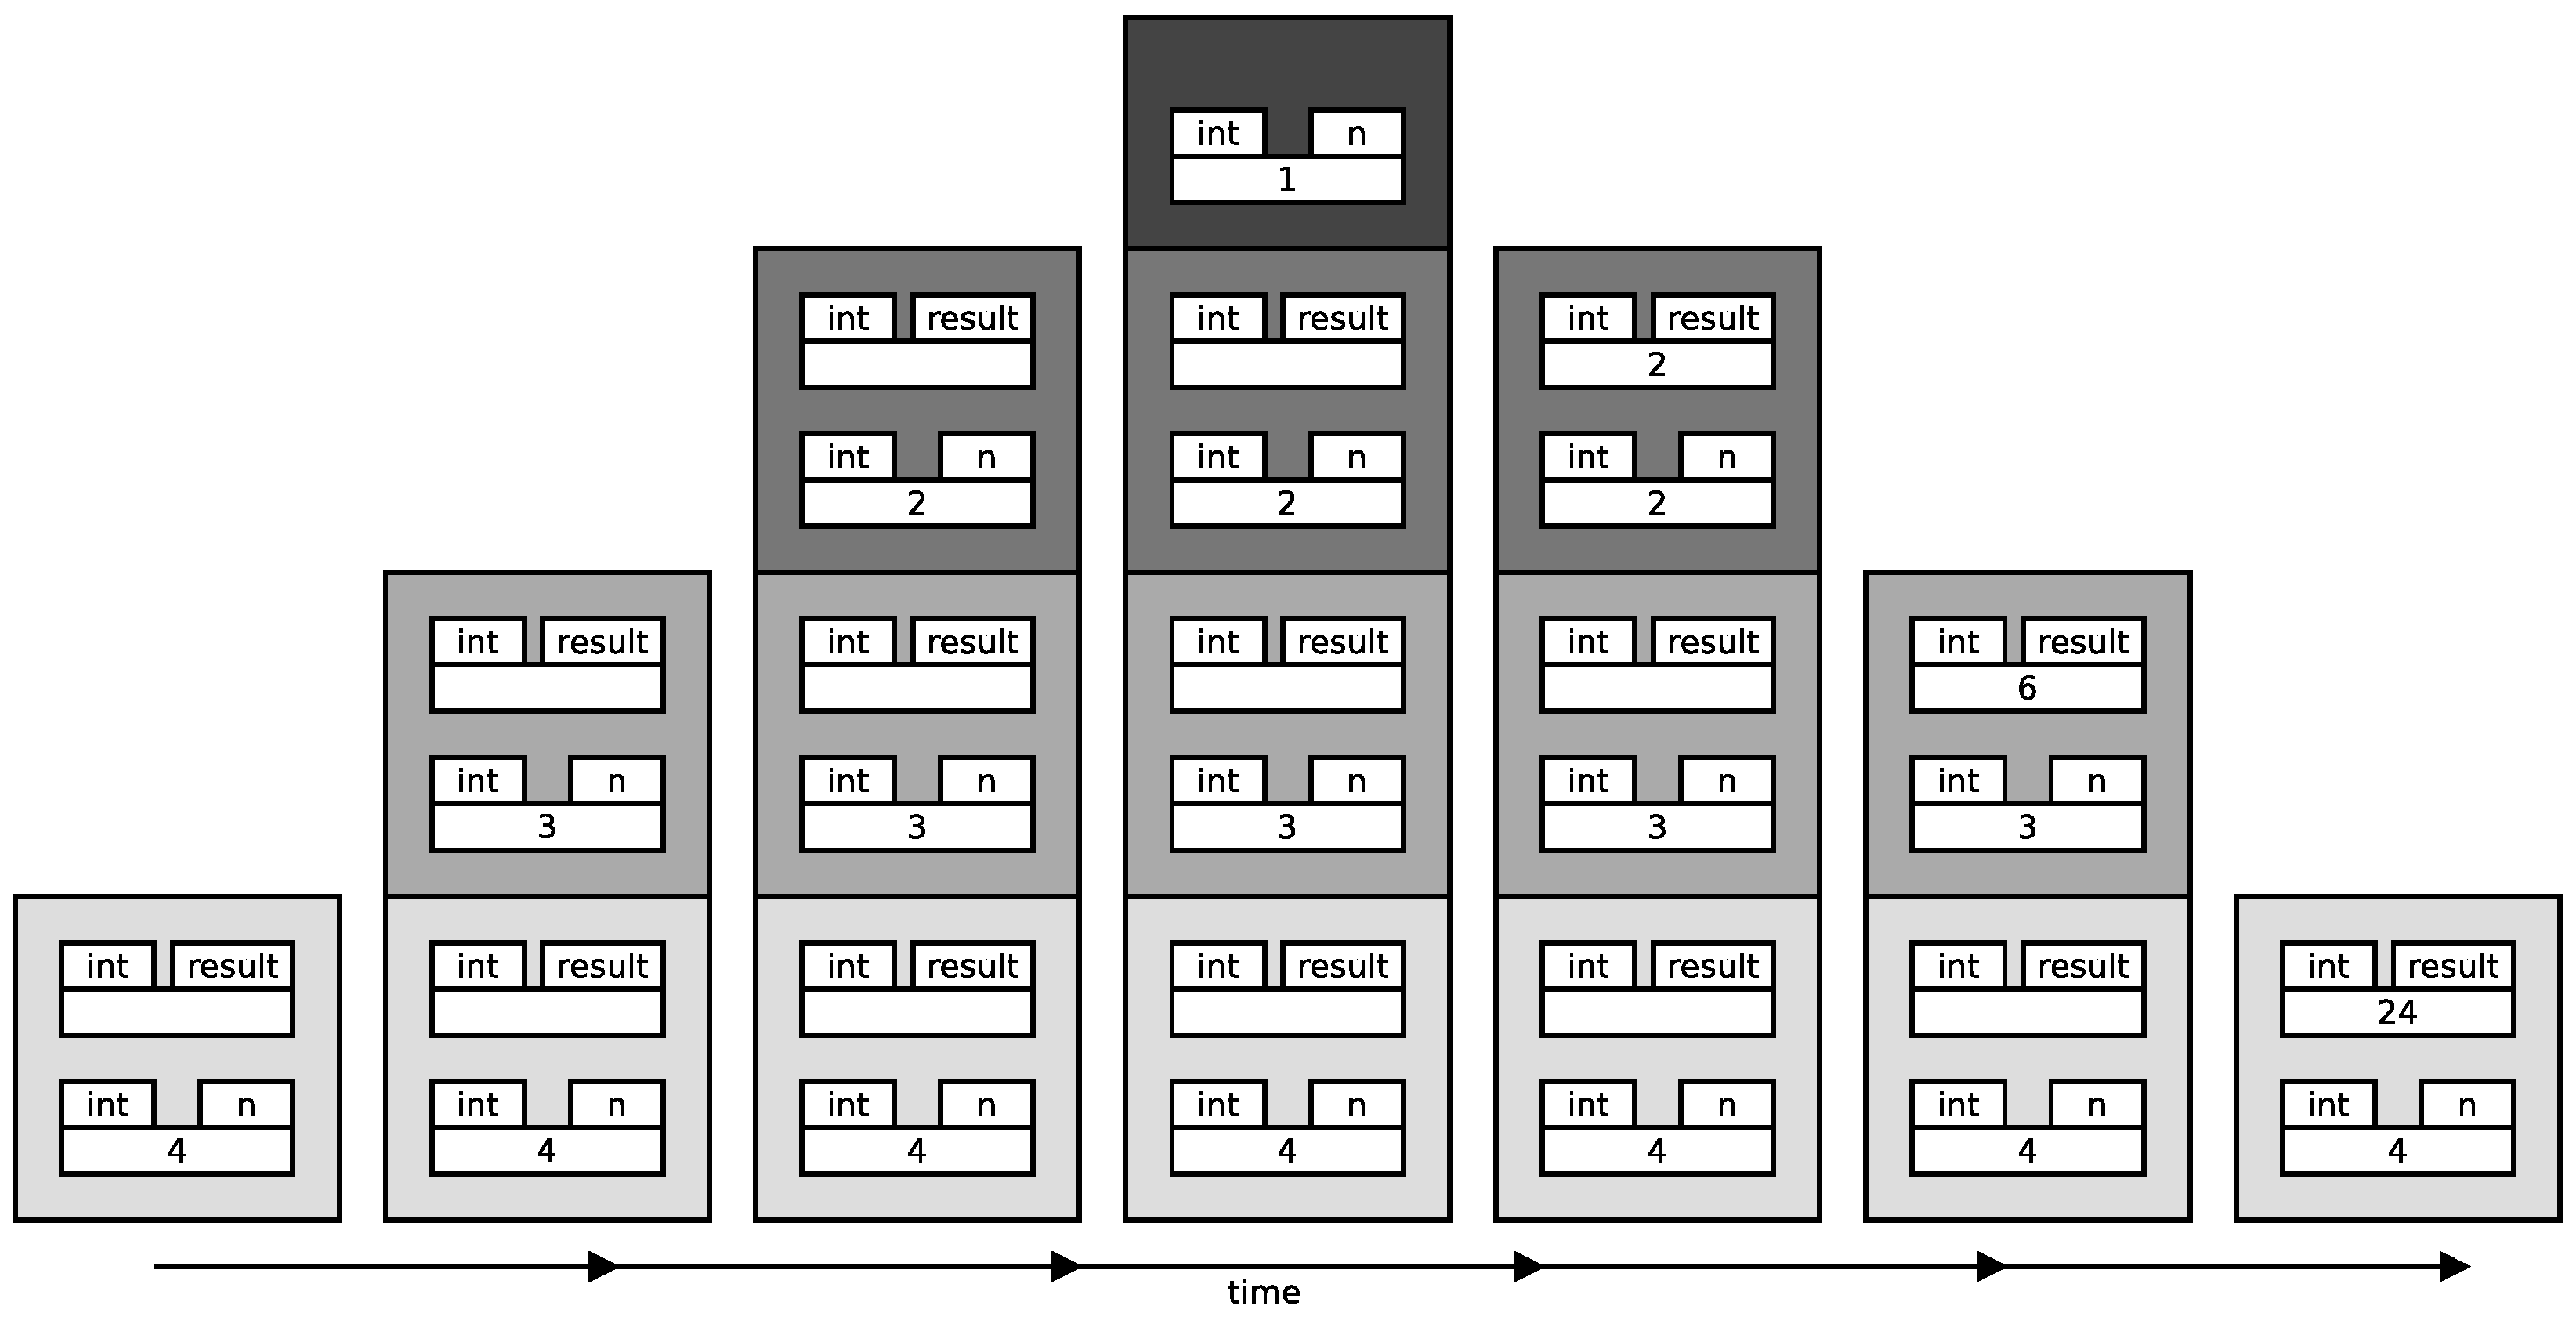
\includegraphics[width=\textwidth]{gfx/recursive-factorial}
  \caption{Evolution of the computer stack when factorial(4) is
    called. Every subsequent call of the method adds a new level to
    the stack, and the variable where the return value will be stored
    is left with an undecided value until the method call returns.}
  \label{fig:fact}
\end{figure}

\subsection{Pitfalls}
\label{sec:pitfalls}

At this point you are familiar with loops (\verb+while+, 
\verb+for+\ldots) and you know that you must be careful with the
way you set the condition of a loop to prevent infinite loops that
block your programs. In a similar way, you must keep in mind a couple
of things when you write recursive code. 

\paragraph{Base case}
\label{sec:base-case}

Every recursive program or method must have a base case for which the
answer is known. In the case of the factorial, we know that~1! is~1;
in the case of the Fibonacci numbers, we know 
that the answer for F(1) and F(2) is~1.
% BAD EXAMPLES NOW THAT LISTS AND TREES HAPPEN AFTER RECURSION-1
%  when we calculate the depth of
% of a tree, we know that the depth of a tree with no descendants is 0;
% when we add a new element to a a list recursively, we know that the
% element will be added to the element were \verb+next+ is pointing to
% \verb+null+. 

If a recursive method does not have a base case, the method will call
itself continuously until the stack is overflown, i.e.~until the
computer tries to add a new level to the stack (to execute the next
method) and finds there is no more memory to do it. At that point, the
Java Virtual Machine will throw a \verb+StackOverflowError+. 

Look at the code on page~\pageref{neverends}. It does not have a base
case, so it will run forever until the computer runs out of memory
space for the stack. 

\paragraph{No convergence}
\label{sec:no-convergence}

Apart from a base case, it is important that each iteration of a
recursive method tries to answer a simpler or more limited version of
the same question. In other words, every time a method is called again
its parameter must be a smaller number, or a shorter list, or ---in
general--- must be nearer to the base case. 

In simple cases like the factorial or the Fibonacci numbers, it is
easy to see that the method will converge. This can be more difficult
when the recursion involves more than one method, e.g.~method A calls
method B, and method B recursively calls A (note than A 
and~B may be methods in
different classes\footnote{A real story: There was a project in which
  we had a window, and inside of it a canvas on which different
  objects were painted. Different elements of the application needed
  to know where the origin was; some of them asked the window and some
  of them asked the canvas. If the window did not know where the
  origin was (e.g.~at initialisation), it asked the canvas. The canvas
  set the origin at initialisation, and informed the window. If the
  user started a new canvas (e.g.~by opening a new file), the new
  canvas did not know the origin but it could ask the window (which was
  already there). All was working well until the first day that a
  user, instead of starting the application and then a file, opened a
  file directly. The file opened in a canvas, that did not know where
  the origin was, so it asked the window; the window had not been told
  where the origin was, so it asked the canvas; and the recursive loop
  continued until the application crashed in front of the eyes of the
  (quite upset) user.}). You must be especially careful when you have
a loop of several methods calling each other recursively because it
may be quite complex to see whether they converge in all cases or not.

If your recursive method does not converge towards a base case, you
will overflow the stack and the Java Virtual Machine will throw a
\verb+StackOverflowError+. 

\subsection{When to use recursion?}
\label{sec:when-use-recursion}

Recursive methods are a way of performing a computation more than
once. In that respect, they are similar to loops. When a problem is
solved by using loops, it is said to be solved \emph{iteratively};
when recursive methods are used, it is solved \emph{recursively}. 

Every problem that can be solved iteratively can be solved
recursively, and viceversa\footnote{This is one of the results of the
 Turing--Church thesis.}. Some programming languages do not have
loops, and some others do not have recursion. Most modern languages,
including Java, Java Decaf, and Groovy have both. 

There is no clear set of rules about when to use one or the other. In
general, recursive code tends to be shorter, simpler, and clearer (but
not always). On the other hand, recursive calls make heavy use of the
stack, which can be an issue in small devices with limited memory. 

As a general rule, you should use whatever you feel is more natural
for the problem at hand. Sometimes the solution to a problem can be
naturally thought in terms of ``if only I had\ldots it would easy
to\ldots''; for example, if you want to build a wall of 100 bricks,
you can think ``if only I had a wall of~99~bricks, it would be easy
to add the~100th~brick''; and if you wanted a wall of~99~bricks, it
would be easy as long as you had a wall made of~98~bricks, and so
on. Then you just need a trivial base case, like ``building a wall 
of~0~bricks'' and you have a recursive solution to your problem. 

You should keep in mind that recursive
solutions are sometimes a bit \emph{harder to think}, 
especially when you are not familiar
with the idea, but they are generally \emph{easier to read}. 
As code is written once but read many times 
(for maintenance, extension, etc), it is usually a good
idea to be a bit biased towards recursive approaches unless the amount
of memory is really limited (and even in that case, remember that
memory and computing power grow every year). 



% Recursion
%   - divide and conquer
%     - example in real life: sorting postal mail (thanks to Knuth)
%     - binary search
%     - quick sort
%     - Advantages: easier to parallelise -> will come to it again



%%% Local Variables:
%%% mode: latex
%%% TeX-master: "d13"
%%% End:
